\documentclass[papersize,30pt,slide]{jsarticle}

\pagestyle{empty}
\usepackage[dvipdfmx]{color}
\usepackage[dvipdfmx]{graphicx}
\usepackage{multicol}

\usepackage{mathpazo}
\usepackage{listings}
\usepackage{jlisting}

\lstdefinelanguage[lisp]{nibkame}{%
   morekeywords={toplet,topletrec,if,match,type,fun}%
   sensitive,% ???
   alsodigit=-+e.,%
   morecomment=[l];,%
   morecomment=[s]{\#|}{|\#},%
   morestring=[b]"%
}[keywords,comments,strings]

\lstdefinelanguage[Objective display]{Caml}[Objective]{Caml}{%
    morestring=[d]',%
%    classoffset=2,
%    morekeywords={int,float,char,string},keywordstyle=\color{red},
%    classoffset=3,
%    morekeywords={list,array},keywordstyle=\color{blue},
%    classoffset=0,
    literate=%
        {[|}{[\hskip -1pt$|$}2%
        {|]}{$|$\hskip -1pt]}2%
%       {[]}{\ensuremath{[\hskip -0.1em]}}2%
        {->}{\ensuremath{\rightarrow}~}2%
        {::}{\ensuremath{:\hskip -0.1em:}~}2%
}
\lstset{language=[Objective display]Caml,%
  basicstyle={\normalfont\normalsize\sffamily},%
  commentstyle={\small\ttfamily\itshape\bfseries\upshape},%
  classoffset=1,%
  keywordstyle={\bfseries},%
  %frame=,%
  %framesep=0pt,%
  showstringspaces=false,%
  %numbers=left,%
  %numberstyle={\scriptsize},%
  %stepnumber=1,%
  tabsize=8,%
  lineskip=-0.5ex,%
%
  breaklines=true,%
  linewidth=\the\textwidth,
%  columns=[l]flexible%
  columns=flexible%
}
\begin{document}
\title{\huge 関数型言語の設計と実装}
\author{
    \Large
    \begin{tabular}{llr}
    L班 & 07317 & 小堀 育男 \\
        & 07322 & 酒本 典明
    \end{tabular}}
\date{}
\maketitle

%\tableofcontents

\section{目的}
教育目的のコンパイラとして開発
\begin{center}
 ML 系関数型言語 Objective Caml のサブセット \\
 MinCaml min-caml.sourceforge.net
\end{center}

「美しい日本の ML コンパイラ」

ただし教育用のサブセット \\
ML としての重要な機能の欠如
\begin{itemize}
\item 多相型
\item 代数的データ型
\item パターンマッチング
\end{itemize}
\begin{center}
 それを補ったコンパイラの作成
\end{center}

\section{プログラム言語 nibkame の設計}
\subsection{構文要素}
\begin{multicols}{2}

組み込みの構文 %\vspace{-0.3cm}
\begin{itemize}
\item 変数への束縛 
\item 条件分岐
\item 関数の生成
\item ヴァリアントの定義
\item パターンマッチング
\end{itemize} 

データ構造 
\begin{itemize}
\item 単純型 \\ int, float, char, bool
\item リスト
\item 配列
\item タプル
\item ヴァリアント
\end{itemize}
\end{multicols}

\newpage
\subsection{What is OCaml?}
\begin{lstlisting}
let max x y =
  if x > y then x else y

let at_least_3 = max 3
\end{lstlisting}
{
実行例:
\begin{tabular}{lcl}
\#\lstinline|max 1 2| &$\Longrightarrow$& 2\\
\#\lstinline|at_least_3 7| &$\Longrightarrow$& 7\\
\#\lstinline|at_least_3 0| &$\Longrightarrow$& 3\\
\#\lstinline|[1; 2; 3]| &$\Longrightarrow$& [1; 2; 3]\\
\#\lstinline|1 :: [1; 2; 3]| &$\Longrightarrow$& [1; 1; 2; 3]\\
\#\lstinline|[1; 2; 3] @ [4; 5]| &$\Longrightarrow$& [1; 2; 3; 4; 5]\\
\#\lstinline|1 :: []| &$\Longrightarrow$& [1]\\
\#\lstinline|1, "abc"| &$\Longrightarrow$& 1, "abc"\\
\end{tabular}

\newpage
}
\subsection*{\thesubsection\quad What is OCaml?}
\begin{lstlisting}
let rec sort xs =
   let rec part pivot hs ls = function
     | [] -> hs, pivot, ls
     | x :: xs ->
       if x > pivot
         then part pivot (x :: hs) ls xs
         else part pivot hs (x :: ls) xs in
   match xs with
     | [] -> []
     | x' :: xs' ->
       let hs, pivot, ls = part x' [] [] xs' in
       sort ls @ pivot :: sort hs
\end{lstlisting}


\newpage
\subsection{基本型}
\begin{tabular}{lcl}
\#\lstinline|1| &$\Longrightarrow$& \lstinline|int|\\
\#\lstinline|[1; 2; 3]| &$\Longrightarrow$& \lstinline|int list|\\
\#\lstinline![|1; 2; 3|]! &$\Longrightarrow$& \lstinline|int array|\\
\#\lstinline|1, 1.0, 'a'| &$\Longrightarrow$& \lstinline|int * float * char| \\
\#\lstinline|max| &$\Longrightarrow$& \lstinline|int -> int -> int|\\
                &$\equiv$& \lstinline|int -> (int -> int)| \\
\#\lstinline|max 1| &$\Longrightarrow$& \lstinline|int -> int|\\
\#\lstinline|max 1 2| &$\Longrightarrow$& \lstinline|int|\\
\end{tabular}

\newpage
\subsection{多相型}
ひとつのプログラムに複数の型がつく

\begin{lstlisting}
val last : 'a list -> 'a
\end{lstlisting}
int list でも char list でも OK

どのような型でも可能なものは, 型変数に置き換わる.\\
使用するときは実際の型が代入される

\vspace{1em}

型推論のおかげで, コンパイラが(C++の)テンプレートのように出来るところを自動で型変数で置き換える

実体化も自動でしてくれる機能

\newpage

\subsection{代数的データ型}
「または」で繋がれたうち, ひとつを取る型 直和型とも

\begin{lstlisting}
type 'a list =
  | Node of 'a * 'a node
  | Null
\end{lstlisting}
これは, \lstinline|list|とは
\begin{itemize}
\item データと次のリストの組であるか
\item 終端である
\end{itemize}
かのいずれかであるということ

この他の状態でないことが保証されたデータ

パターンマッチとの組み合せが強力

\newpage
\subsection{クロージャ}
関数と, それの実行に必要なものをひとまとまりにしたもの
関数引数の他に, 外から与えられる自由変数をあわせたもの

\begin{verbatim}
cf. グローバル変数
\end{verbatim}
呼び出したときでなく, 関数の書かれた位置で値が決まる

\begin{lstlisting}
  let g y =
    let h z = y + z in
    h in
  let h' = g 1 in
    h' x    (* x+1 *)
\end{lstlisting}
関数 \lstinline|g| をでたのに \lstinline|y| の値が参照できる!

\newpage
\subsection{パターンマッチング}
データの構造を記述し, 直接取り出す

いちいち
\begin{lstlisting}
let first = nth 0 list
let second = nth 1 list
let others = drop 2 list
\end{lstlisting}
ではなく
\begin{lstlisting}
let fist :: second :: others = list
\end{lstlisting}
と, 左辺に構造(パターン)を書き, 右辺と同じ造りにする

\newpage
\subsection{パターンマッチングとヴァリアント}
左辺に相当するものを複数書くこともできる \\
先のヴァリアントと組み合せて
\begin{lstlisting}
match list with
  | Node (1, tail) ->
    先頭のデータが 1 だったとき
  | Node (head, tail) ->
    データが存在するとき
  | Null ->
    末尾であったとき
\end{lstlisting}
のような場合分けもできる

型システムから, 出現しうるパターンを予測できる 

\hspace{1em} $\rightarrow$ パターンに漏れがないか検査できる

\section{コンパイラの構造}

\begin{itemize}
\item 構文解析とS式表現での出力 
\item S式表現の読み込み
\item 型推論
\item パターンマッチングの展開
\item K正規化
%\item 名前付け替え, インライン展開, 簡約
\item クロージャ変換
\item 仮想機械語へ変換
\item 仮想機械語の線形化
\item x86命令の生成
\item レジスタ割り当て
\item アセンブリコードの出力
\end{itemize}

\newpage

\subsection{構文解析}
解析表現文法を用いた構文解析器 \\
Schemeにて実装

%マクロの実装はこの段階で行う

\subsection{S式表現}
\begin{lstlisting}
let rec gcd = fun x y ->
  if y = 0 then x else gcd y (x - y)
\end{lstlisting}

\begin{lstlisting}[language=Lisp,columns=fullflexible,morekeywords={topletrec,fun,if},deletekeywords={gcd}]
(topletrec gcd
  (fun (x y)
    (if (= y 0)
      x
      (apply gcd y (- x y)))))
\end{lstlisting}

\newpage
\subsection{型推論}
わかっている型を探し,構文から同じであるべきところ同士を単一化していく
\begin{lstlisting}
定数 -> 型は自明
変数 -> 環境から探す
関数 ->
  引数に型変数を当てて本体の型を求め, 組み合せる
関数適用 ->
  結果となる型変数を用意し,関数と引数の型を求め,
  関数の型と,引数から結果への関数型とで単一化する
分岐 -> 分岐先ふたつの型を求め,単一化する
変数束縛 ->
  束縛する値の型を求め,その型を用いて続く式を推論する
\end{lstlisting}

\newpage
\subsection{K正規化}
計算のオペランドが変数と定数が二つになるようにする

計算機の多くでは,二つしかソースにとれない. \\
そういった機械語に近づける操作

\subsection{クロージャ変換}
ネストした関数は全てトップレベルに括り出す

自由変数が出現する場合には, 関数の定義された場所をクロージャ変数の生成に置き換える

ないのならば, 呼び出しは他の関数と同じにできる

\newpage

\subsection{仮想機械語の生成}
計算機の命令として一般的なものと,組込み関数として実現するものを分けてい
く.レジスタにある変数と,メモリに置かれるデータの区別を始める.

\subsection{仮想機械語の線形化}
ここまでは,命令は木構造をしている.それを単純な並びに直し,ジャンプ命令
を挿入する.

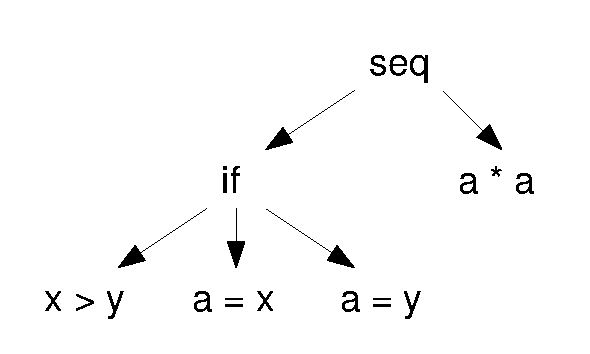
\includegraphics[scale=0.3]{instree.pdf}
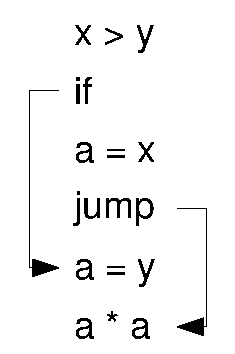
\includegraphics[scale=0.3]{insliner.pdf}

\subsection{命令選択}
線形化した仮想機械語を x86 命令に置き換えていく

この段階では変数は全てレジスタに置かれているとする

\subsection{レジスタ割り当て}
実際に変数へレジスタを割り当てる

スタックフレームの生成と破棄はここで挿入される

\section{付録}
\subsection{メモリへのデータ構造の割り付け}
動的なデータの割り付け先
\begin{itemize}
\item 基本的なサイズのリスト
\item float型を格納するリスト
\item その他 タプルと配列, クロージャ
\end{itemize}
ヴァリアントは基本サイズのリストと同様に割り付け

多分にGCを搭載することを意識している

\newpage
\subsection{リストの構造}
\begin{lstlisting}[language=C]
struct list {
    dword data;
    void *next;
}
\end{lstlisting}
また, 基本サイズのリストはデータが参照であるかどうかを示すビットマップを持つ

\vspace{1em}

ヴァリアントは \\
データ部にタグ番号を, ポインタに持つべきデータへの参照
としてリストと同様に配置

\newpage
\subsection{タプルと配列}
タプル

\includegraphics[scale=0.7]{tuple.pdf}

ヘッダには
\begin{itemize}
\item 参照を示すビットマップ
\item タプルのデータの個数
\end{itemize}
が格納される

大きなタプルは分割して, 末尾を続きへの参照とする

\newpage

配列

\includegraphics[scale=0.7]{array.pdf}

サイズはデータの個数 最上位ビットは参照かどうか

\vspace{1em}

ヘッダ部分はGCしか(おそらく)使わないので, オフセットの計算が容易になるよう変数の値はデータ部を指すようにした

\vspace{1em}

クロージャ変数 \\
関数へのポインタと自由変数のタプル

\end{document}
